\newpage

\section{How to request an IPA Account / VPN Access for Cerro Pachon Services}
  
  To request an IPA account, it is required for the user to create a Service Request ticket inside the IT User Support Dashboard.
  Please check the example below.

  Head over to https://jira.lsstcorp.org and log in with your domain account credentials.

\vspace{5 mm}

\begin{figure}
  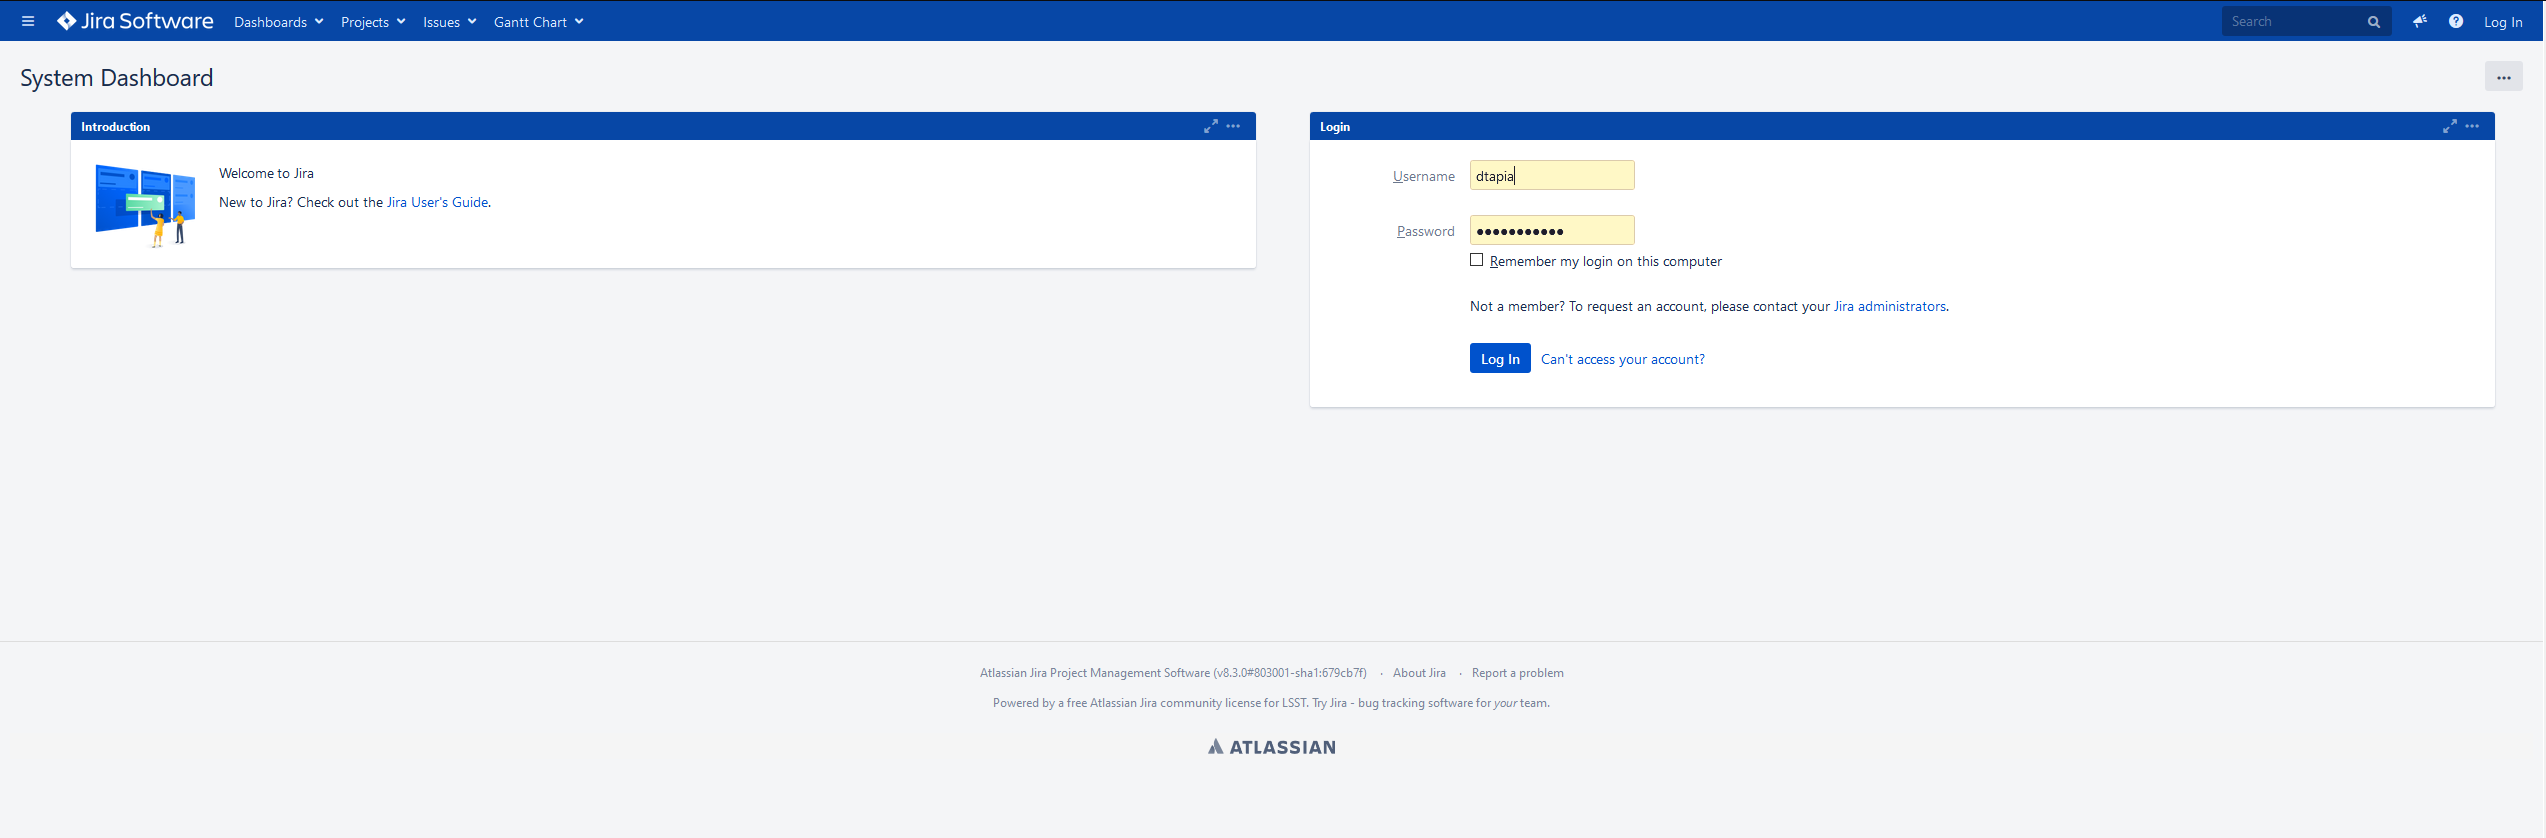
\includegraphics[width=12cm]{Images/example1.png}
\end{figure}

\vspace{5 mm}

Once logged in the user will be prompted with the following windows if not similar. Before creating the ticket,  it is required for the user to check that he is in the proper dashboard for this particular case the IT Support Dashboard

\vspace{5 mm}

\begin{figure}
  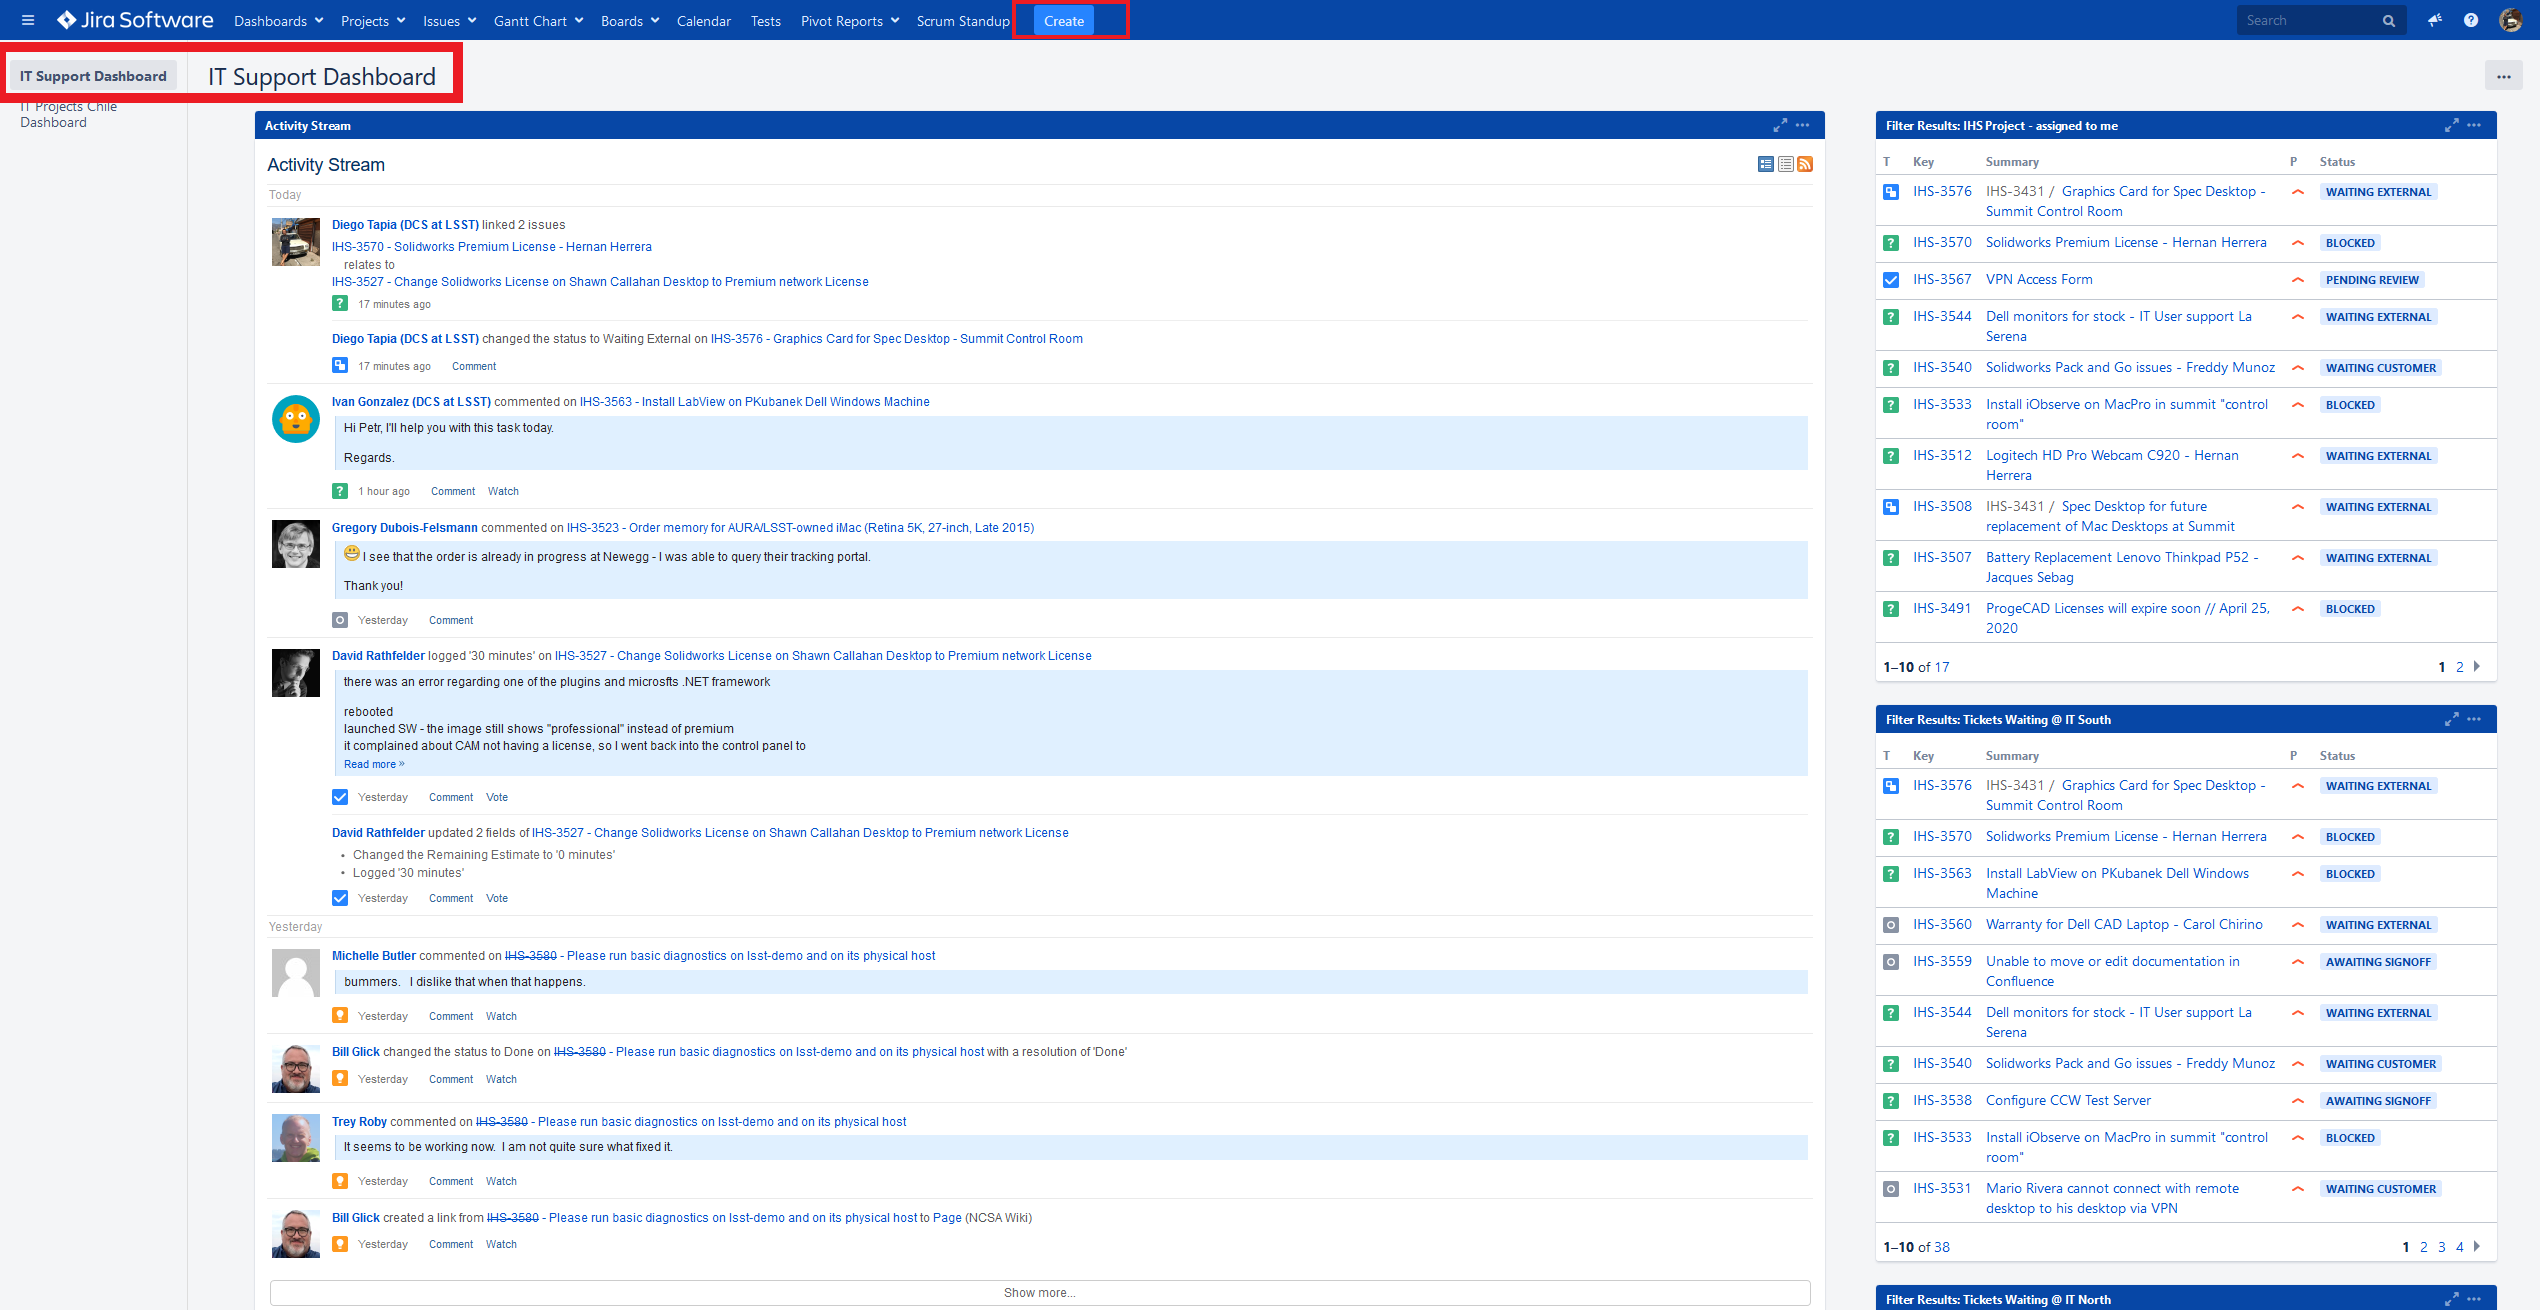
\includegraphics[width=12cm]{Images/example2.png}
\end{figure}

\vspace{40 mm}

On the ticket creation window fill out the template using the information provided below:

\begin{itemize}
  \item Project: IT Helpdesk Support (IHS)
  \item Issue Type: Service Request
  \item Summary: IPA Account Creation / VPN Access - "Insert your name here"
  \item Component: AAA
  \item Description: Please use the template provided below.
\end{itemize}

\vspace{10 mm}

\begin{figure}
  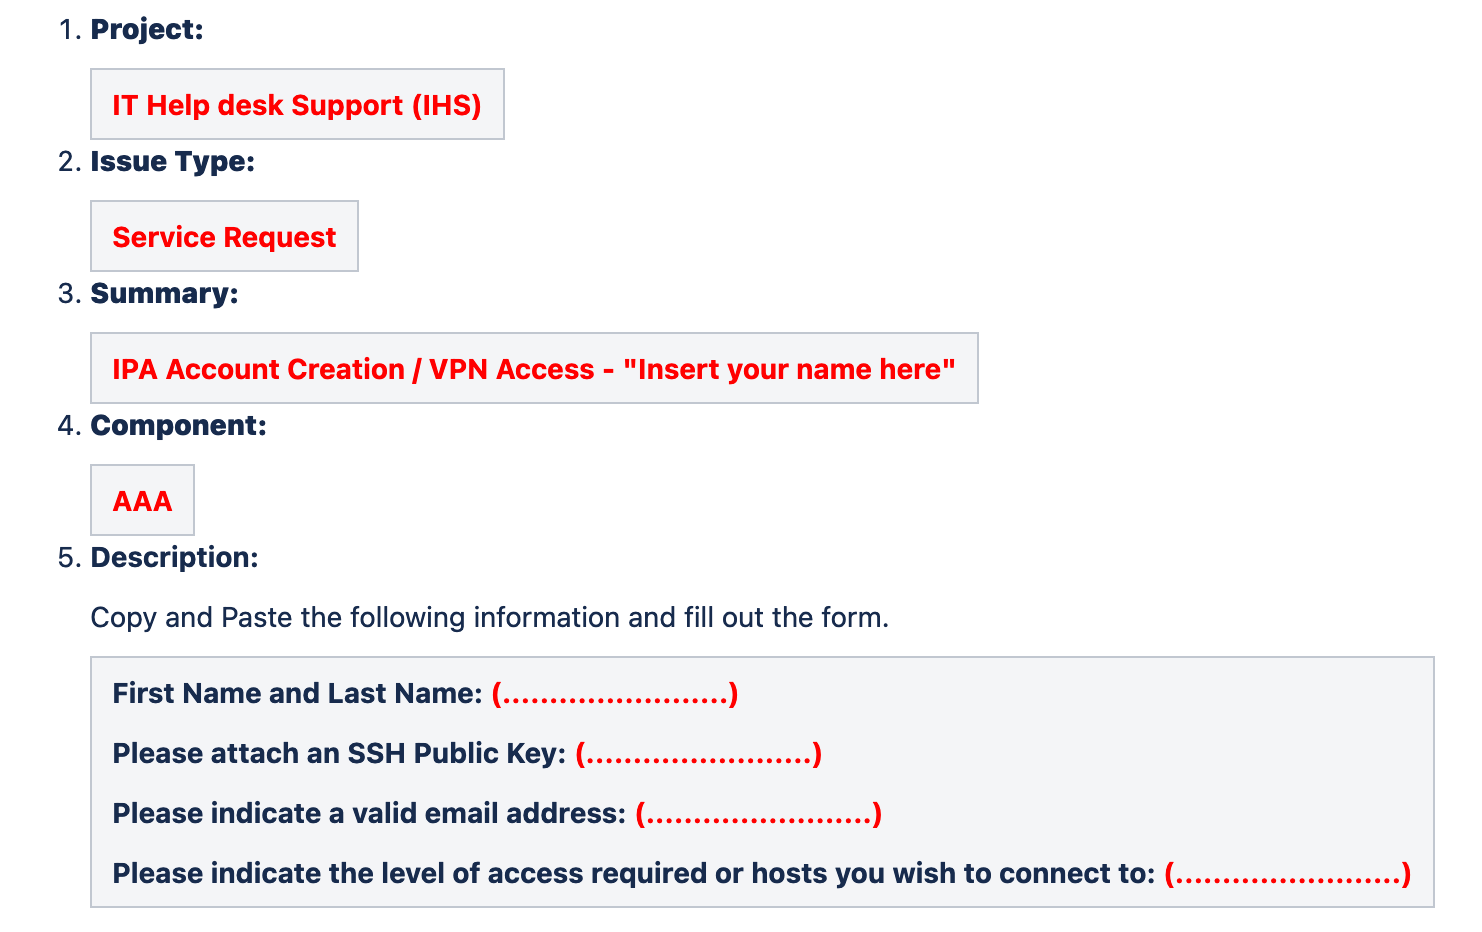
\includegraphics[width=15cm]{Images/example4.png}
\end{figure}

\newpage

Once all the information is filled out, select the Create option located at the bottom to create the ticket inside IHS IT Support Dashboard.

\vspace{10 mm}

\begin{figure}
  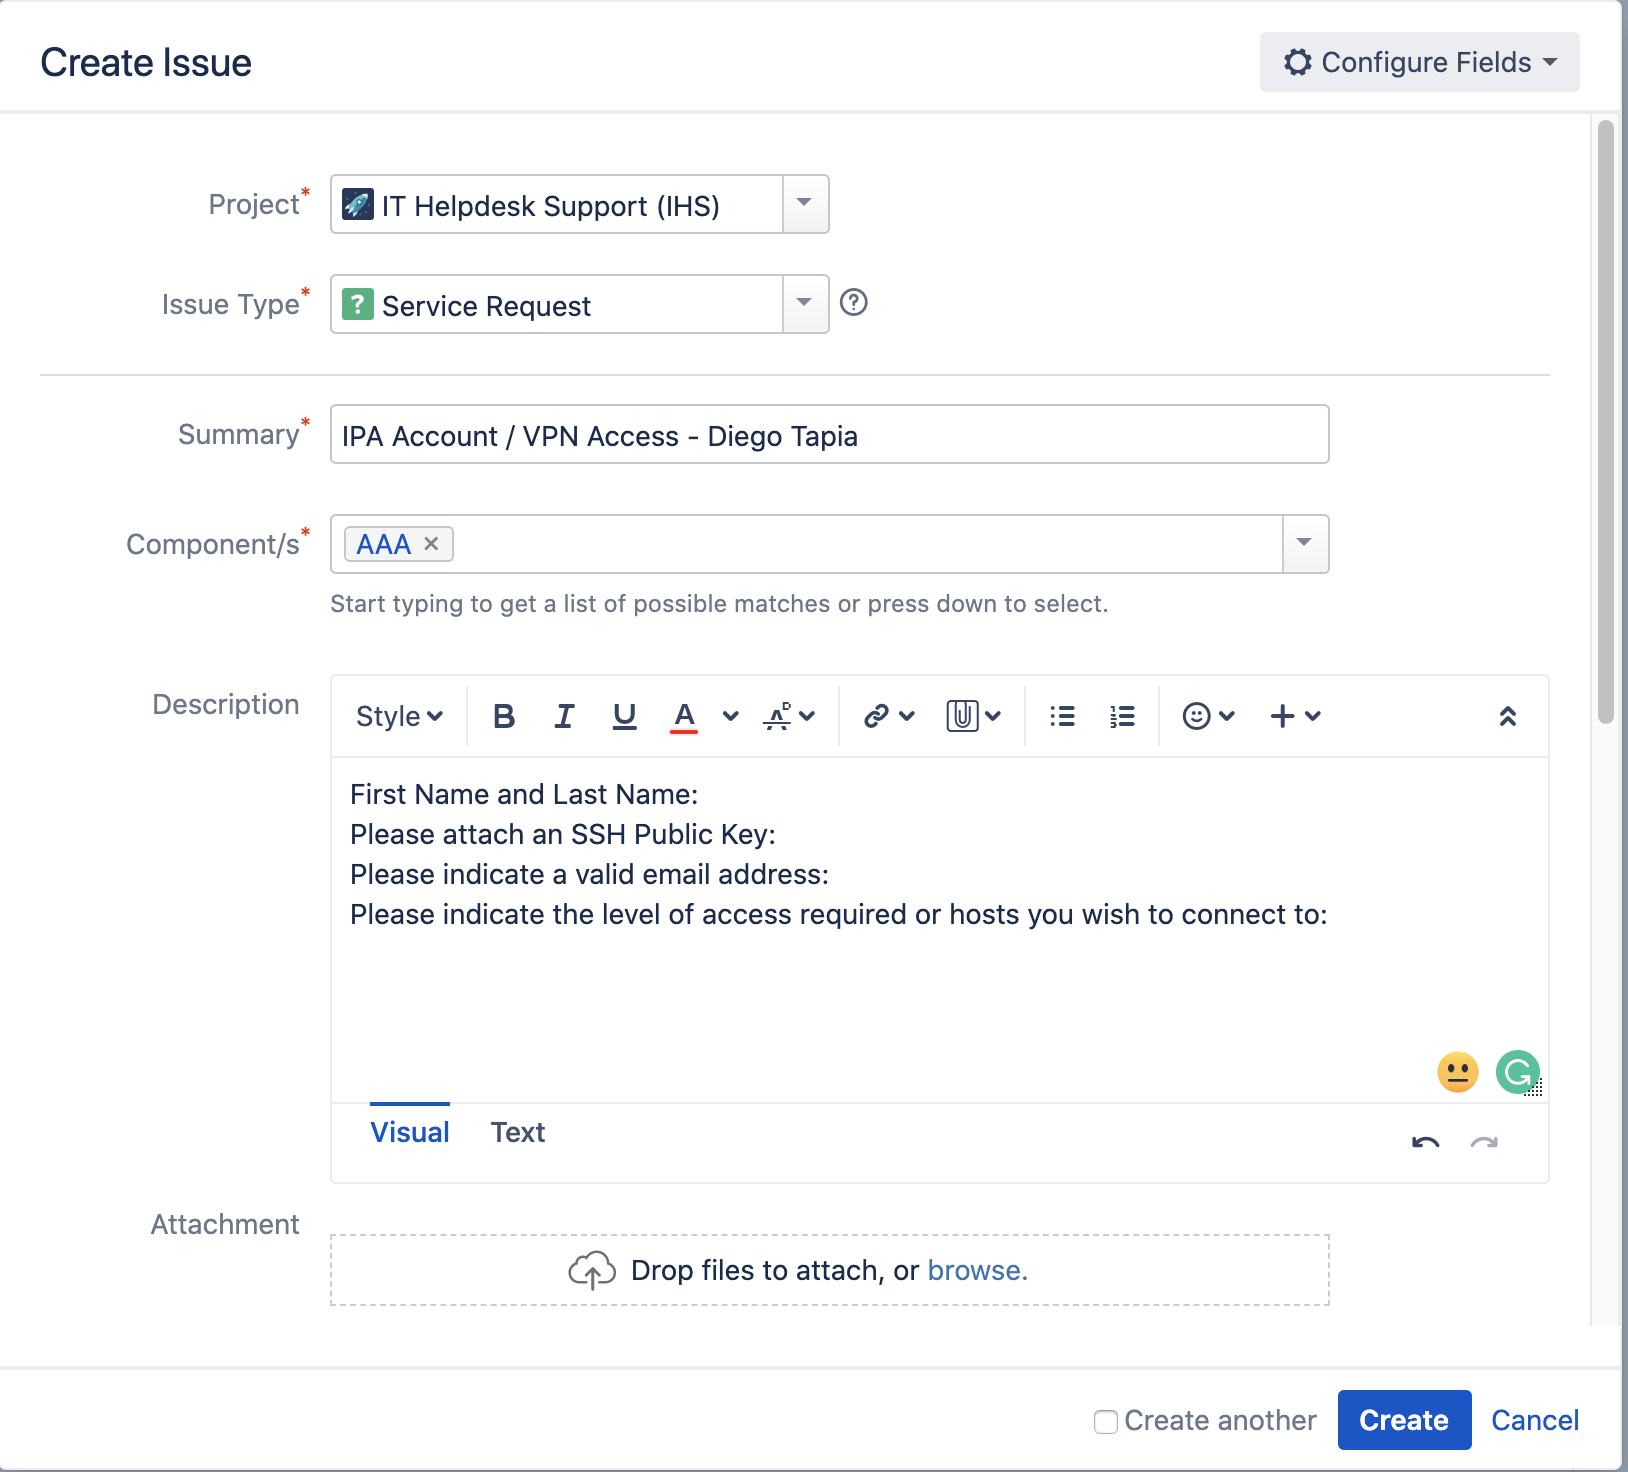
\includegraphics[width=13cm]{Images/example3.png}
\end{figure}

\vspace{10 mm}
IT User support will receive the request and will proceed with the account creation process. Once the account has been created and the services have been provisioned IT Support will be in contact with you via email to provide you with the account credentials and services you've been granted access too along with the website where you can change your temporary password.

IF you have any questions or concerns regarding the services provisioned please contact IT User Support at rubinobs-it-las@lsst.org
